% !TEX root = ../paper_zh.tex

\section{UAV-TAlign-12K 与评测协议}

\subsection{数据集范围}

UAV-TAlign-12K 是面向真实无人机红外-可见光对齐的基准。数据集包含 6,039 对同步 RGB-红外
图像，对应 15 个场景中的 12,078 张图像。正式评测划分包含 6,037 对经过完整性检查的图像，
共计 12,074 张。数据覆盖跨视场与跨分辨率感知条件，包括白天、夜间和低照度采集，灰度与伪彩
热成像渲染，以及广角、变焦和常规无人机视图。

所有期刊规模实验均使用同一个版本化 manifest。UAV-TAlign-1K-Lite 保留为固定的开发与消融
子集，而 UAV-TAlign-12K 用于本文的基准规模评测。正式划分包含 7 个白天场景、5 个夜间场景
和 3 个低照度场景，同时包含 8 个灰度热成像场景和 7 个伪彩热成像场景。变电站场景族中的成对
广角与变焦视图提供了受控的跨视场比较。

\begin{table}[t]
\caption{UAV-TAlign-12K 与代表性红外-可见光及无人机多模态资源的定位比较。UAVMatch 表示采用
合成变换监督的无人机对齐基准。}
\label{tab:dataset_positioning_zh}
\centering
\resizebox{\textwidth}{!}{
\begin{tabular}{lllll}
\toprule
资源 & 数据基础 & 对齐信号 & 规模 & 主要评测重点 \\
\midrule
KAIST / FLIR / LLVIP / M3FD & 地面或混合 RGB-红外数据 & 成对或已对齐影像 & 依数据集而定 & 检测、融合、低照度感知 \\
DroneVehicle / VTUAV / LasHeR / Anti-UAV & 无人机或跟踪型 RGB-红外数据 & 任务标注 & 依数据集而定 & 多模态检测或跟踪 \\
UAVMatch / TGRS~\cite{gao2025uavmatch} & 无人机多模态数据的合成变换 & 仿射 / 单应性监督 & 81K 训练 / 15K 测试对 & 监督式变换回归与几何指标 \\
ATR-UMMIM~\cite{bin2025atrummim} & 真实无人机可见光 / 红外 / 已配准可见光三元组 & 半自动像素级参考 & 7,969 个三元组 & 成对配准精度与条件属性 \\
UAV-TIRVis~\cite{vasile2025uavtirvis} & 真实无人机热红外-可见光影像 & 人工成对配准 & 80 对 & 直接图像域配准质量 \\
UAV-TAlign-12K & 真实采集跨视场无人机红外-可见光数据 & 多帧场景协议 & 6,039 个候选 / 6,037 个评测对 & 成对证据、场景共识与运行覆盖率 \\
\bottomrule
\end{tabular}}
\end{table}

\begin{figure}[t]
\centering
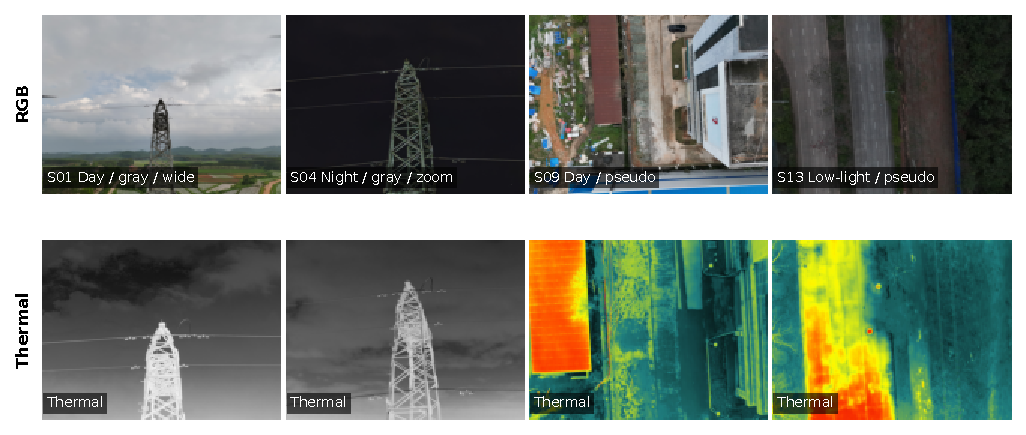
\includegraphics[width=\textwidth]{figures/fig_dataset_examples.pdf}
\caption{UAV-TAlign-12K 的代表性 RGB-红外图像对，覆盖不同光照、热成像渲染和视图条件。}
\label{fig:dataset_examples_zh}
\end{figure}

\subsection{采集与整理}

UAV-TAlign-12K 的采集时间跨度为 2024 年下半年至 2026 年上半年，覆盖中国南部的工业与自然
场景。全部场景均使用同一套 DJI Matrice 350 RTK 平台和 Zenmuse H30T 多传感器载荷采集。
集成载荷自动同步可见光与红外产品，从而保留原生跨传感器几何关系。飞行方式包括悬停和航线式
采集，所用无人机完成实名登记，飞手具有 CAAC 资质，并在允许飞行的空域内执行任务。

发布的数据流保留 H30T 原生采集模式。广角相机静态图像分辨率为 $4032\!\times\!3024$，变焦
相机静态图像为 $3664\!\times\!2748$，热红外图像为 $1280\!\times\!1024$。场景 01 和 02 的
$3840\!\times\!2160$ 静态图像是在 H30T 录像期间触发拍照获得。场景 07 是同步视频抽帧序列，
以每秒 2 帧的频率采样，覆盖无人机环绕输电塔一周的完整过程。灰度场景使用 H30T 的
\emph{White Hot} 设置，伪彩场景使用设备内置的 \emph{Hot Iron} 色板。

数据整理标准在算法评测前冻结，涵盖场景相关性、曝光、对焦和文件完整性。整理后的候选数据集
包含 6,039 对同步图像，完整性审计进一步定义了 6,037 对正式评测划分。筛选过程不使用匹配器
输出、对齐估计或质量分数。

发布准备阶段移除嵌入式元数据并规范化文件名，同时保持图像像素不变。RGB 与红外文件通过共享
的 H30T 采集键关联，按采集时间与序列索引排序，并赋予共同的六位图像对标识。发布过程不进行
缩放、裁剪、旋转、重压缩或图像增强。数据集归广西大学所有，并计划采用知识共享署名 4.0 国际
许可协议发布。

\subsection{数据组织}

每个场景均包含独立的 \texttt{rgb/} 与 \texttt{thermal/} 目录，配对样本具有相同的文件名主干。
正式 manifest 记录场景标识、图像对标识、光照条件、热成像渲染、视图类型和场景标签。一个场景
用于汇集具有共同地点或目标语境及采集条件的帧，可以来自连续序列，也可以来自同一场景定义下的
多次架次。场景 07 是明确记录的单次环绕视频序列。

同一个 manifest 支撑全部成对、场景和条件分析，并把每一项报告结果映射回对应场景与图像对标识。

\subsection{多层评测协议}

基准定义三个互补轨道。轨道 A 独立评测全部 6,037 对图像，衡量成对单应性证据的可用性与支撑度。
轨道 B 将逐帧估计聚合为场景变换，并报告规范定义的高置信场景产品集合。轨道 C 使用固定、可解释
的可靠性分数对场景排序，从而构建覆盖率感知的运行曲线。

三个轨道共同把匹配器输出与可部署场景几何联系起来。成对指标刻画证据生成，场景级指标刻画
多帧共识，运行曲线则反映场景质量变化时产品覆盖率的演变。

\subsection{无标注场景一致性诊断}

该协议采用无标注相对信号进行可扩展的场景一致性分析。所存储的诊断量比较优化后变换与基线初始
变换，并量化跨模态一致性的变化，包括边缘重叠增益、梯度 NCC 增益、梯度一致性改善帧比例、
严重基线相对离群点数量与比例、接受帧支撑、单应性离散度，以及鲁棒剔除比例。

这些信号共同刻画跨模态改善、几何支撑和共识稳定性，并通过统一评测接口支撑规范产品选择、条件
感知分析和可靠性--覆盖率可视化 \cite{ma2021survey,liao2024survey}。
